\subsection{Non-linear sloshing in a rectangular container}%Ansari

Free surface oscillations of a liquid confined in a closed container (sloshing phenomenon) are an important issue when big amounts of liquid are industrially transported. The phenomenon involves two fluids that share a free surface boundary separating them, normally the density of the upper fluid is several orders of magnitude less than the bottom one. This phenomenon has proven of great interest due to the fact that violent impacts of the fluid can affect the structural integrity of the container.

For the studied cases, the sloshing phenomenon is produced by a horizontal harmonic excitation $x = a_h (\sin \omega_h t)$, where $a_h$ is the excitation amplitude and $\omega_h$ is the excitation frequency of the rectangular tank where the two fluid phases are contained. The tank is divided in two parts, the bottom part is water with a density of $\rho_{I} = 1000 [kg/m^3]$ and the top part contains a fluid
with different densities $\rho_{II} = 1.3, 50, 200, 800 [kg/m^3]$, depending on the case studied\cite{Goni13}. The dimensions of the
tank are $a$(width) by $b$(height) and the initial free surface is at height $h$ from the bottom of the tank, see Figure \ref{fg:ansari-config}. The free surface starts the simulation as a horizontal line and is subsequently deformed by the tank excitation and the flow dynamics.

\begin{figure}[H]
  \begin{center}
      \includegraphics[width=.7\columnwidth]{images/ansari_config.pdf}
  \end{center}
  \caption{\label{fg:ansari-config} Configuration scheme of the Non-linear sloshing in a rectangular container case. Initial condition is represented by dotted lines.}
\end{figure}

For the different cases in this report, a 2D rectangular tank $a=1.0[m]$ width by $b=1.0[m]$ height is used. The initial height of the interface is $h=0.5[m]$ and the lateral excitation applied is $x=0.05\sin(3t)$. The simulations were performed considering the
flow as laminar and non-viscous, hence no turbulence model was used and slip boundary conditions are taken. Density was modified according to the considered ratios $\sigma=\frac{\rho{II}}{\rho{I}}$. A two dimensional Cartesian mesh of $450\times225$, splitted into triangles, has been used in all cases.

Reference results for this case are taken from \cite{Goni13} which uses the codes STARCCM+ and \OF to obtain numerical solutions and reports the free surface displacement on the left wall of the container. Those simulations use the same grid as presented above, but, in order to avoid numerical instabilities, they limit the $CFL$ number to $CFL_{max}=0.5$. In PFEM-2 simulations do not exist that restriction then $\Delta t$ is fixed to $0.1$, reaching $CFL_{max}\approx5$.

  \begin{figure}[h]
  \centering
    \subfloat[]{
	  \label{fg:ansari-1}         %% Etiqueta para la primera subfigura
	  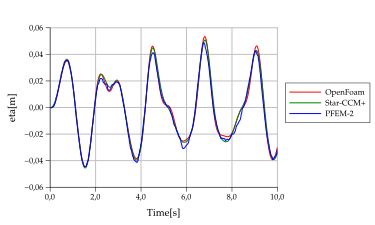
\includegraphics[width=.8\columnwidth]{images/ansari_1.pdf}
    } \\
    %%----segunda subfigura----
    \subfloat[]{
	  \label{fg:ansari-2}         %% Etiqueta para la segunda subfigura
	  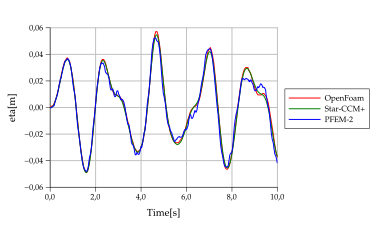
\includegraphics[width=.8\columnwidth]{images/ansari_2.pdf}
    } \\
    \subfloat[]{
	  \label{fg:ansari-3}         %% Etiqueta para la primera subfigura
	  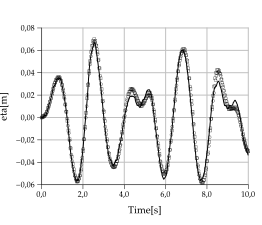
\includegraphics[width=.8\columnwidth]{images/ansari_3.pdf}
    } \\
    %%----segunda subfigura----
    \subfloat[]{
	  \label{fg:ansari-4}         %% Etiqueta para la segunda subfigura
	  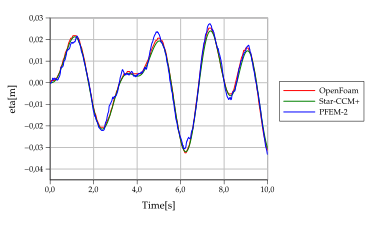
\includegraphics[width=.8\columnwidth]{images/ansari_4.pdf}
    }
   \caption{Sloshing comparison for a two phase flow for different density ratios. Figure \ref{fg:ansari-1}: $\sigma=0.0013$, Figure \ref{fg:ansari-2}: $\sigma=0.05$, Figure \ref{fg:ansari-3}: $\sigma=0.2$ and Figure \ref{fg:ansari-4}: $\sigma=0.8$.
}
   \label{fg:ansari-results}                %% Etiqueta para la figura entera
\end{figure}

Figure \ref{fg:ansari-results} presents results with different density ratios. For each one of them, PFEM-2 simulations shows a good agreement with reference solutions, further more considering that the time step used is around five to ten times bigger.
\clearpage
\subsection{Viscous standing waves}%Re=250,2500.

Computing the dissipation due to wave-breaking remains a challenging problem in the computational fluid mechanics context. In order to analyze the solution with PFEM-2 of two-phase viscous incompressible flows, the evolution of a viscous standing wave has been chosen. This is a classical problem in the scientific literature for which an approximate analytical solution is available for small amplitude perturbations\cite{Lighthill01} and it is of practical interest since it is related to the propagation of gravity waves.

The chosen standing wave configuration consists in a rectangular tank with length $L$ and a water filling height of $H = L/2$. This setup is taken from \cite{Colagrossi12}, and in the Figure \ref{fg:standing-wave-config} a sketch of this configuration is displayed. The wave length is $\lambda = L$, $k$ is the corresponding wave number (i.e. $k = 2\pi/\lambda$), $A$ is the wave amplitude and denotes the ratio $\epsilon=2A/H$.

\begin{figure}[H]
  \begin{center}
      \includegraphics[width=.9\columnwidth]{images/standing_wave.pdf}
  \end{center}
  \caption{\label{fg:standing-wave-config} Configuration scheme of standing wave case. Initial condition is represented by dotted lines. In continuous line is presented an intermediate state where the maximum amplitude $A$ is reached.}
\end{figure}

If the fluid is viscous, the dissipation due to the solid boundary layers is neglected, small-amplitude waves (i.e small $\epsilon$) and small wave steepness (i.e $2A/\lambda \ll 0.1$) are used; an approximate analytical solution of the standing wave evolution can be obtained through the linearization of Navier-Stokes equations for traveling waves:
\begin{align}
 \varphi(x,y,t) & = \varphi_0(x,y)\cos(\omega t) \\
 \varphi_0(x,y) & =-\epsilon\frac{Hg}{2\omega}\frac{\cosh\left[k(y+H)\right]}{\cosh(kH)}\cos(kx)
\end{align}

where the circular frequency $\omega$ is given by the dispersion relation of gravity waves, that is, $\omega^2 = g k \tanh(kH)$ where $g$ is the acceleration of gravity. At time $t = 0$ the free surface is horizontal while the initial fluid velocity is given by $\varphi_0$.

It can be demonstrated that the approximate solution is well posed only for $Re\gg1$ and for $Re^{-1}\ll k \ll Re^{2/3}$, where $Re=H\sqrt{gH}/\nu$ is the Reynolds number for this problem. From that solution, it is possible to obtain the formula that gives the approximate decay of the kinetic energy\cite{Lighthill01}:

\begin{equation}
 \varepsilon_K(t) = \epsilon^2g\frac{\lambda H^2}{32}e^{-4\nu k^2t}\left[1+\cos(2\omega t)\right]
 \label{kin-eq}
\end{equation}

The kinetic attenuation is governed by the coefficient of the exponential $\beta_l = 4\nu k^2$, which depends on the wave number and on the kinematic viscosity $\nu = \mu/\rho_{I}$. Lately work\cite{Antuono13} has demonstrated that generally, the Equation \ref{kin-eq} overestimates the dissipations, especially when the Reynolds number is not very large. Then an improved damping rate is proposed in that paper $\beta = 4\nu k^2 -  2\sqrt{2}k^{11/4}Re^{-3/2}+O(Re^{-2})$, which is next used for comparisons.

To accomplish the linear solution hypothesis, the PFEM-2 simulations have been implemented by using a free-slip condition for the velocity and a Neumann condition for the pressure along each boundary of the tank. Also, the parameters $L=2$, $A=0.05$ and $g=1$ have been selected.

Several Reynolds number ($Re=25,50,250,2500$) have been selected to compare with the approximate analytic dissipation. Problems were solved into a grid with $H/\Delta x=100$ and varying $\Delta t$ in order to solve using a Fourier number $Fo=\frac{\nu\Delta t}{\Delta x^2}$ with a local maximum of $Fo_{max}\approx10-50$. Figure \ref{fg:sw-energy} shows the comparison between the expected dissipation (which includes the improving damping rate) and numerical results with PFEM-2. Large Fourier numbers were used in order to reduce the computation times required to complete the simulations and to show the accuracy of the method working not only with large CFL numbers, even with large diffusion rate.

  \begin{figure}[h]
  \centering
    \subfloat[]{
	  \label{fg:sw-energy-25}
	  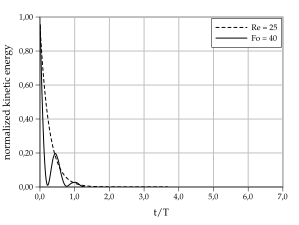
\includegraphics[width=.72\columnwidth]{images/sw_25.pdf}
    } \\
    \subfloat[]{
	  \label{fg:sw-energy-50}
	  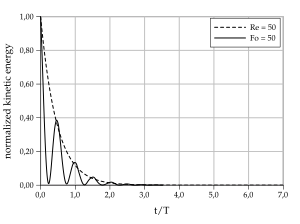
\includegraphics[width=.72\columnwidth]{images/sw_50.pdf}
    } \\
    \subfloat[]{
	  \label{fg:sw-energy-250}
	  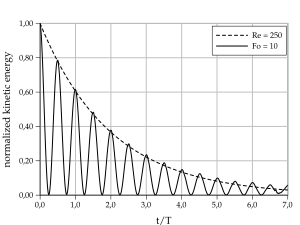
\includegraphics[width=.72\columnwidth]{images/sw_250.pdf}
    } \\
    \subfloat[]{
	  \label{fg:sw-energy-2500}
	  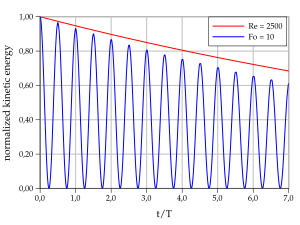
\includegraphics[width=.72\columnwidth]{images/sw_2500.pdf}
    }
   \caption{Kinetic Energy decay for standing wave problem with different Reynolds numbers. Red lines are approximate analytical solutions for total energy and blue lines are numerical solutions with PFEM-2. Reynolds numbers analyzed: $Re=25,50,250,2500$ in Figures \ref{fg:sw-energy-25},\ref{fg:sw-energy-50},\ref{fg:sw-energy-250},\ref{fg:sw-energy-2500} respectively. Legend in each figure indicates the maximum Fourier number used in each numerical simulation.}
   \label{fg:sw-energy}
\end{figure}
% \afterpage{\clearpage}
\subsection{Rayleigh-Taylor Instability}

This problem consists on the evolution of two layers of fluids initially at rest in the gravity field. The top layer is more dense than the one is placed at the bottom. Due to a little disturbance in the contact surface the more dense fluid goes down and the less dense fluid does the opposite. In the intermediate state a mixture is created, which is lately segregated. The final state reaches an stable equilibrium with the more dense fluid at the bottom layer and the less dense fluid at the top layer. The growth and evolution of the instability has been investigated among others by Tryggvason\cite{Tryggvason88} for inviscid incompressible flows, and by Guermond
\& Quartapelle\cite{Guermond00} for viscous flows.

The starting point is the problem documented by Guermond. The domain is $[−d/2,-2d]\times[d/2,2d]$. The initial position of the perturbed interface is $\eta(x) = −0.1d \cos(2\pi x/d)$. The heavy fluid is above and the density ratio is $3$, so that the Atwood
number is $0.5$ according to Tryggvason's definition $At = (\rho_{max}-\rho_{min})/(\rho_{max}+\rho_{min})$. Other physical parameters are selected to obtain $Re=\rho_{min}d^{\frac{3}{2}}g^{\frac{1}{2}}/\mu=1000$. Computational domain is discretized into $160000$ structured triangles ($\Delta x=0.01$) setting slip boundary conditions on each wall. Time step selected is $\Delta t=0.01[s]$, which allows to reach $CFL_{max} \approx 8$.

To compare with reference results, the time is made dimensionless by using $\widetilde{t} = t\sqrt{g\ At}$. Results on the vertical position of the tip of the falling and rising fluid (spike and bubble, respectively) are shown in Figure \ref{fg:rayleigh-rf}. It can be observed that current solution is in good agreement with the reference results.

\begin{figure}[H]
  \begin{center}
      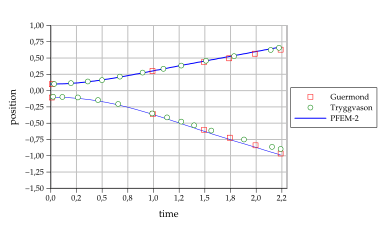
\includegraphics[width=\columnwidth]{images/rayleigh_1.pdf}
  \end{center}
  \caption{\label{fg:rayleigh-rf} Position of rising and falling bubbles versus time. Case with $Re=1000$.}
\end{figure}

On the other hand, the evolution of the instability is shown in Figure \ref{fg:rayleigh-screenshots} at dimensionless times $\widetilde{t}=0, 1, 1.5, 2$. Around $\widetilde{t}=1.5$ the heavy fluid begins to roll up into two counter-rotating vortices. Later, around $\widetilde{t} = 2$, these two vortices become unstable and a pair of secondary vortices appear at the tails of the roll-ups. These shapes of the fluid interface obtained with PFEM-2 are similar than those of the reference results.


\begin{figure}[htbp]
  \begin{center}
      \includegraphics[width=\columnwidth]{images/rayleigh_2.jpg}
  \end{center}
  \caption{\label{fg:rayleigh-screenshots} Rayleigh-Taylor instability evolution. Case with $Re=1000$. From left to right $\widetilde{t} =0.0$, $1.0$, $1.5$, $2.0$.}
\end{figure}
\afterpage{\clearpage}
\subsection{Sloshing roll.}%ETSIN experimental tests

\subsection{Dam-break problem}%ETSIN experimental tests

The objectives of this section are to compare experimental measurements on dam-break flow over a dry horizontal bed with the numerical approximation carried out with the pfem algorithm. The extensive set of experimental data is extracted from \cite{Lobovsky13}, where the dynamics of the dam break wave impacting a vertical wall downstream the dam, with emphasis on the pressure loads and surface evolution after the dam burst, are presented.

Computational configuration of the tank used in experimental cases is presented in Figure \ref{fg:dambreak-config}. There, the locations of water level measuring points and pressure sensors are shown. In this report only the case with $H=300[mm]$ is analyzed. Two-phase non-viscous flow simulation is carried on, with $\rho_{water}=1000[kg/m^3]$ and $\rho_{air}=1[kg/m^3]$ with a gravity force $\mathbf{g}=-10\ \hat{j} [m/s^2]$. The 2D computational grid used has $322\times120$ nodes, conforming a mesh with around $80000$ triangles. Boundary conditions are slip on all walls, and $\Delta t$ is fixed to $0.1$, which allows to reach $CFL_{max}\approx20$ when free surface impacts the downstream wall.

\begin{figure}[htbp]
  \begin{center}
      \includegraphics[width=\columnwidth]{images/dam_break_config.pdf}
  \end{center}
  \caption{\label{fg:dambreak-config} Configuration scheme of the dam-break case. $H_1$, $H_2$, $H_3$, $H_4$ present the locations of water level measuring positions. Also, $P_1$, $P_2$, $P_3$, $P_4$ show the locations of pressure sensors at the impact wall downstream the dam. Grey zone represents the initial condition. Dimensions in millimeters.}
\end{figure}

Figure \ref{fg:dambreak-h} shows the comparison between experimental and numerical results for each water-level measurement. A good agreement can be observed, moreover taken into account the capture of the back wave and splashing start events.
  \begin{figure}[h]
  \centering
    \subfloat[]{
	  \label{fg:dambreak-h1}         %% Etiqueta para la primera subfigura
	  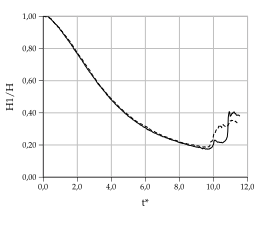
\includegraphics[width=.48\columnwidth]{images/dambreak_h1.pdf}
    }
    %%----segunda subfigura----
    \subfloat[]{
	  \label{fg:dambreak-h2}         %% Etiqueta para la segunda subfigura
	  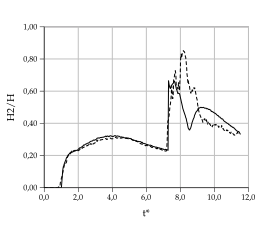
\includegraphics[width=.48\columnwidth]{images/dambreak_h2.pdf}
    } \\
    \subfloat[]{
	  \label{fg:dambreak-h3}         %% Etiqueta para la primera subfigura
	  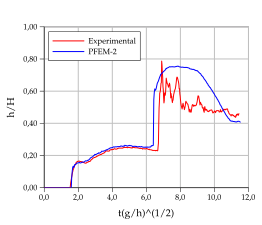
\includegraphics[width=.48\columnwidth]{images/dambreak_h3.pdf}
    }
    %%----segunda subfigura----
    \subfloat[]{
	  \label{fg:dambreak-h4}         %% Etiqueta para la segunda subfigura
	  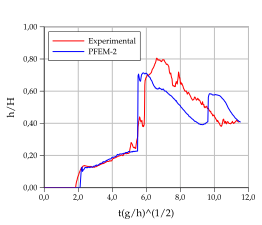
\includegraphics[width=.48\columnwidth]{images/dambreak_h4.pdf}
    }
   \caption{Water level elevations at locations $H_1$, $H_2$, $H_3$ and $H_4$ for tests with $H=300[mm]$ initial filling height compared to data from literature experimental results\cite{Lobovsky13} and numerical results with PFEM-2.}
   \label{fg:dambreak-h}                %% Etiqueta para la figura entera
\end{figure}

The impact pressure was measured with four sensors at the vertical wall at the end of the downstream flume, as described in Figure \ref{fg:dambreak-config}. The statistical analysis of the pressure peaks, rise times and the occurrence time, i.e. the time between
the opening of the dam gate and the occurrence of the impact, is presented in Figure \ref{fg:dambreak-p}. The shown pressure $P$ is non-dimensionalized with regards to the hydrostatic pressure at the bottom of the reservoir and denoted as $P^∗$.

In the reference work, the analysis is focused on peaks events. It can be noticed that the highest peak is recorded by sensor number 1 which is the sensor receiving the full impact, whilst the pressure of the other sensors is given by the run up of the flow. It can also be observed that sensor number 4, i.e. the sensor located at the highest position, does not show a pure impact event, see Figure \ref{fg:dambreak-p4}, and actually the maximum for this sensor is obtained later in time, when the water falls back after running along the wall. Numerical solution behavior follows the mentioned conclusions, but the pressure values are not between the statistical limits of experimental data. Also, a discrepancy can be observed with the peaks times for sensors $1$ to $3$. This difference can be assigned to the numerical simplification which does not model the gate movement.

  \begin{figure}[h]
  \centering
    \subfloat[]{
	  \label{fg:dambreak-p1}         %% Etiqueta para la primera subfigura
	  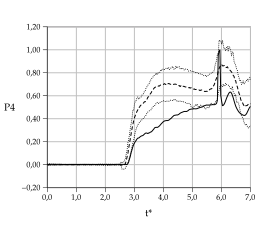
\includegraphics[width=.48\columnwidth]{images/dambreak_p4.pdf}
    }
    %%----segunda subfigura----
    \subfloat[]{
	  \label{fg:dambreak-p2}         %% Etiqueta para la segunda subfigura
	  \includegraphics[width=.48\columnwidth]{images/dambreak_p3.pdf}
    } \\
    \subfloat[]{
	  \label{fg:dambreak-p3}         %% Etiqueta para la primera subfigura
	  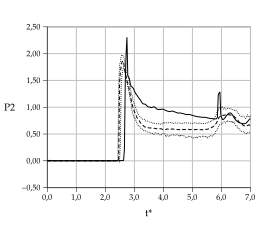
\includegraphics[width=.48\columnwidth]{images/dambreak_p2.pdf}
    }
    %%----segunda subfigura----
    \subfloat[]{
	  \label{fg:dambreak-p4}         %% Etiqueta para la segunda subfigura
	  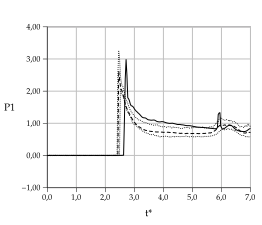
\includegraphics[width=.48\columnwidth]{images/dambreak_p1.pdf}
    }
   \caption{Pressure time histories comparison between experimental results\cite{Lobovsky13} and numerical results with PFEM-2. Locations $P_1$, $P_2$, $P_3$, $P_4$ area presented in Figures \ref{fg:dambreak-p1},\ref{fg:dambreak-p2},\ref{fg:dambreak-p3},\ref{fg:dambreak-p4} respectively. Experimental results shows the median and percentiles $2.5$ and $97.5$.}
   \label{fg:dambreak-p}                %% Etiqueta para la figura entera
\end{figure}

  \begin{figure}[H]
  \centering
    \subfloat[]{
	  \label{fg:dambreak-1}
	  \includegraphics[width=.48\columnwidth]{images/dambreak_pfem_1.jpg}
    }
    %%----segunda subfigura----
    \subfloat[]{
	  \label{fg:dambreak-2}
	  \includegraphics[width=.48\columnwidth]{images/dambreak_pfem_2.jpg}
    } \\
    \subfloat[]{
	  \label{fg:dambreak-3}
	  \includegraphics[width=.48\columnwidth]{images/dambreak_pfem_3.jpg}
    }
    %%----segunda subfigura----
    \subfloat[]{
	  \label{fg:dambreak-4}
	  \includegraphics[width=.48\columnwidth]{images/dambreak_pfem_4.jpg}
    }\\
        \subfloat[]{
	  \label{fg:dambreak-5}
	  \includegraphics[width=.48\columnwidth]{images/dambreak_pfem_5.jpg}
    }
    %%----segunda subfigura----
    \subfloat[]{
	  \label{fg:dambreak-6}
	  \includegraphics[width=.48\columnwidth]{images/dambreak_pfem_6.jpg}
    } \\
    \subfloat[]{
	  \label{fg:dambreak-7}
	  \includegraphics[width=.48\columnwidth]{images/dambreak_pfem_7.jpg}
    }
    %%----segunda subfigura----
    \subfloat[]{
	  \label{fg:dambreak-8}
	  \includegraphics[width=.48\columnwidth]{images/dambreak_pfem_8.jpg}
    }
   \caption{Snapshots of the dam-break at times $t=0,0.25,0.5,0.75,1,1.25,1.5,1.75[s]$.}
   \label{fg:dambreak-screenshots}
\end{figure}
\clearpage
% \subsection{Shear layer flow.}